
\begin{wrapfigure}{R}{0.5\textwidth}
\centering
\begin{subfigure}{.5\textwidth}
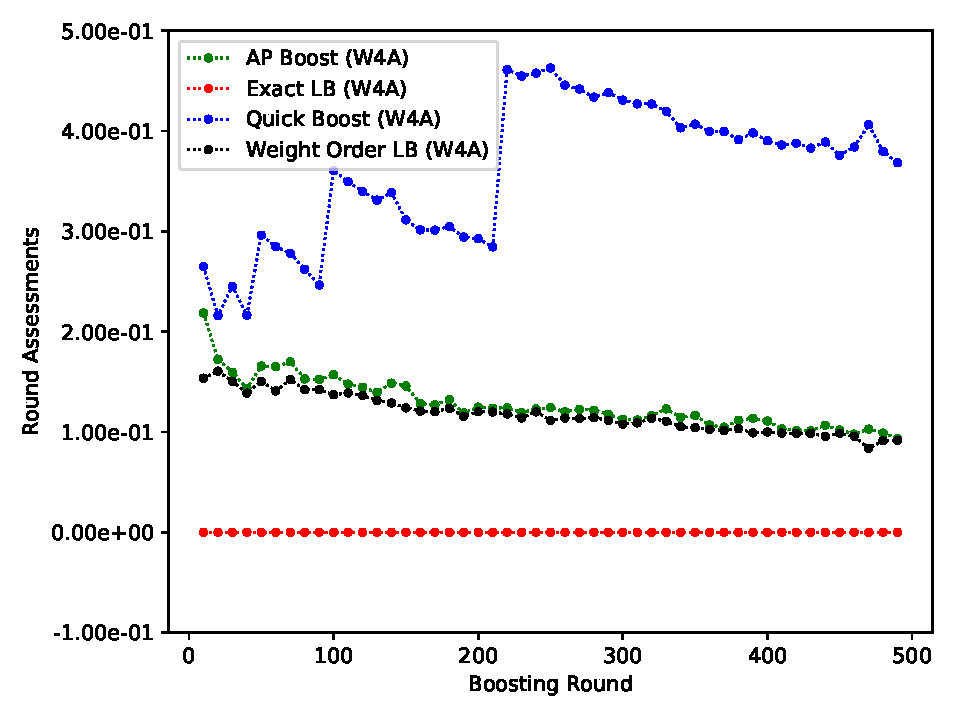
\includegraphics[width=\linewidth]{decisiontree/figures/result4_elb_w4a}
\end{subfigure}
\begin{subfigure}{.5\textwidth}
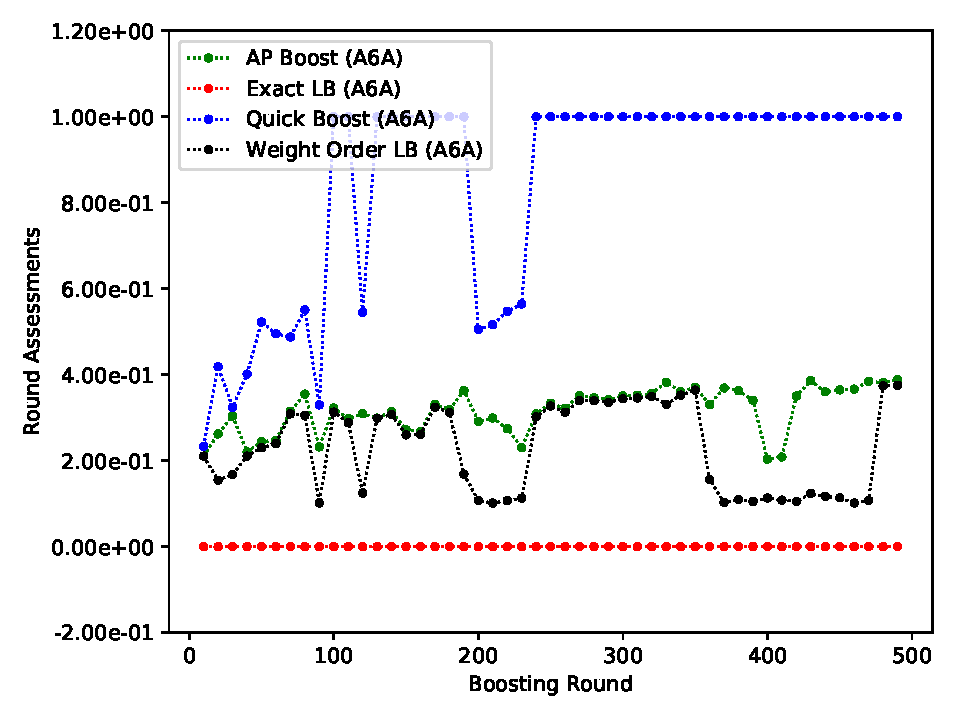
\includegraphics[width=\linewidth]{decisiontree/figures/result4_elb_a6a}
\end{subfigure}
\caption{Lower Bounds versus Upper Bounds. Datasets W4A (top) and A6A (bottom) were used with trees of depth 1.
The y-axis is the \emph{fraction of the gap}
between the exact lower bound
(at zero) and the full corpus size (at one) which an algorithm used in a
given round.
Non-cumulative example assessments are plotted for every 10 rounds.
}
\label{fig:elb}
\vspace{-2em}
\end{wrapfigure}
